\documentclass[letterpaper,journal,10pt]{IEEEtran}

\usepackage{amsmath,amssymb}
\usepackage{graphicx}
\usepackage{booktabs}
\usepackage{cite}
\usepackage{balance}
\usepackage{url}
\usepackage{textcomp}
\usepackage{stfloats}
\usepackage{newtxtext,newtxmath}

\title{Predictability-Aware Soft Set Hopping Against Reactive Jamming}
\author{Tong~Chen, Rui~Zhang, and Lihong~Mao%
\thanks{This work was supported by the Xinjiang Vocational University of
Technology Research Fund under Grant XGZDZK202509. \textit{(Corresponding
author: Tong Chen.)}}%
\thanks{Tong Chen is with the School of Electronic and Information Engineering,
Beijing Jiaotong University, Beijing 100044, China, and also with Xinjiang
Vocational University of Technology, Kashgar, Xinjiang 844004, China (e-mail:
chenton0501@gmail.com). Rui Zhang and Lihong Mao are with Xinjiang Vocational
University of Technology, Kashgar, Xinjiang 844004, China.}}

\begin{document}
\maketitle

\begin{abstract}
Hard recent-set exclusion in sparse multicarrier frequency hopping
creates a predictable boundary spike:
$C_{L_h+1}=S/(N-L_hS)$ grows with memory depth, and
probability-aware exposure equals this height. We propose
predictability-aware soft hopping with capped inclusion probabilities
(PASH-cap), using soft penalties and a probability cap that bounds
worst-case exposure. On a coded OFDM grid, PASH-cap reduces BLER from
$0.138$ (MCSH-L2) to $0.020$ at delay three; against a causal attacker with 12
candidate lags, BLER is $0.045$ versus $0.126$ for MCSH-L2, with BLER $0.039$--$0.047$ under degraded feedback.
Five online-learning variants all sustain BLER $0.454$--$1.000$.
\end{abstract}

\begin{IEEEkeywords}
Anti-jamming communications, frequency hopping, OFDM, reactive jamming,
predictability, boundary spike, probability cap.
\end{IEEEkeywords}

\section{Introduction}
\IEEEPARstart{F}{requency-hopping} (FH) links evade reactive jammers by varying their occupied
frequencies, but a history-aware jammer can exploit structure in the hopping
rule itself. This problem is practically relevant: in tactical and vehicular
networks, a sparse multicarrier waveform must maintain connectivity under a
follower jammer that tracks spectral occupancy, and set-valued hopping is a
natural fit for these bandwidth-efficient links. Recent defenses encompass index-modulated FH
\cite{shi2022enhanced}, data-driven and reinforcement learning (RL) hopping
\cite{zhou2024,zhang2024block,qi2024,cheng2025,chen2026dual}, anti-jamming games
\cite{zhang2024game}, and jamming-modulation schemes \cite{ma2023}.
Detection-focused work addresses reactive jammer identification in OFDM
\cite{altun2022reactive,wesolowski2023detection} and cooperative sensing
\cite{li2024}. Sequence constructions provide wide-gap or no-hit-zone
properties \cite{shu2024widegap,zheng2025widegap}, while coded OFDM studies
emphasize receiver-side mitigation \cite{mailaender2013,kaplan2023,chen2023,mendonca2024channel,wu2026llr}.
These approaches broadly share a design philosophy of \emph{avoiding} recent
frequency usage, whether through combinatorial sequence constraints or learned
policies.

This letter examines a different question: when recent frequency sets
are excluded too aggressively, what structural consequence does that exclusion
itself create? Most existing work assumes that stronger avoidance of recent
usage monotonically improves anti-jamming performance. We show that this
assumption fails in a precise and quantifiable way. Hard exclusion guarantees
zero collision with a follower whose delay falls within the protected memory,
but it also shrinks the conditional choice space, making frequencies just
beyond that memory disproportionately likely to reappear. We prove that the
collision probability at the first unprotected lag is
$C_{L_h+1}=S/(N-L_hS)$, which grows toward unity as the protected memory
deepens. This is not an engineering tradeoff that could be eliminated by a
better hard-exclusion design; it is a structural consequence of the
zero-collision guarantee itself (we refer to this hard memory-constrained
set hopping scheme as MCSH throughout). Moreover, the same concentration makes the conditional
inclusion probabilities maximally informative to a probability-aware attacker:
the candidate-aware exposure equals the boundary-spike height, so deeper
memory simultaneously raises the worst-case predictability cost.

This diagnostic result distinguishes our work from the existing literature.
Wide-gap and no-hit-zone constructions provide deterministic pairwise
collision-avoidance at specified delays \cite{shu2024widegap,zheng2025widegap},
but they target FH patterns with one active subcarrier per symbol ($S=1$) and do
not address the conditional-inclusion concentration that arises under set-valued
hopping with $S>1$ active subcarriers. RL-based policies can learn to avoid
recent frequencies through online collision feedback \cite{zhou2024,zhang2024block},
but they offer no interpretable bound on the exposure they create, and their
closed-loop nature introduces a vulnerability to feedback manipulation that we
show empirically. Rather than optimizing a hopping policy, we diagnose
a structural consequence of memory and provide a tunable open-loop alternative
that avoids the convergence pitfalls of online learning.

Building on this diagnosis, we propose predictability-aware soft hopping with
capped inclusion probabilities (PASH-cap). It replaces hard exclusion with
exponential penalties on recent subcarrier use and enforces a per-subcarrier
probability cap $p_{\max}$ through systematic sampling. The cap directly bounds
the worst-case conditional exposure: $R_{\mathrm{cand}}\leq p_{\max}$, in
contrast to MCSH where $R_{\mathrm{cand}}=S/(N-L_hS)$ is unbounded.
PASH-cap is open-loop (requires no jammer feedback), incurs no learning
latency, and cannot be manipulated through corrupted or falsified collision feedback.

This letter makes three contributions. First, we derive the collision at the
first unprotected lag of MCSH and prove
that the boundary-spike magnitude $S/(N-L_hS)$ follows unavoidably from the
zero-collision guarantee; deeper memory amplifies rather than removes the
exposure. Second, we propose PASH-cap with an explicit inclusion-probability
cap, implemented by a fixed-size sampler that preserves target marginals
exactly. Third, we evaluate five methods spanning the key design dimensions of
open-loop set-valued FH (Random, BCD, LFSR, MCSH, PASH-cap) under fixed-delay,
probability-aware, and feedback-aided causal attacks, plus a 5-variant
$\times$ 4-threat online-learning matrix confirming that closed-loop
strategies without anti-predictability control fail systematically.

\section{System and Threat Model}
In symbol $m$, the transmitter activates
$\mathcal A_m\subseteq\{1,\ldots,N\}$, where $|\mathcal A_m|=S$. A jammer
occupies an equal-size set $\mathcal J_m$, and the normalized collision is
\begin{equation}
 c_m=\frac{|\mathcal A_m\cap\mathcal J_m|}{S}.
\end{equation}
Define the lag-$d$ self-collision
$C_d=\mathbb E[|\mathcal A_m\cap\mathcal A_{m-d}|/S]$. A fixed-delay follower
uses $\mathcal J_m=\mathcal A_{m-d}$, so its expected collision equals $C_d$.
We test $d=1$ and $d=3$. Two deterministic constructions are included
as structural stress cases that span the design space: a block-cyclic
deterministic construction (BCD) that cycles through $N/S$ orthogonal
sets ($C_1{=}\cdots{=}C_7{=}0$, $C_8{=}1.0$), and a linear-feedback-shift-register (LFSR) based
pseudorandom construction representing the classical FH strategy of
tactical systems ($C_d{\approx}S/N$, but $R_{\mathrm{cand}}{=}1.0$ because the
conditional marginals remain deterministic, $p_{k,m}{\in}\{0,1\}$).

The probability-aware attacker knows the conditional marginals
$p_{k,m}=\Pr(k\in\mathcal A_m\mid\mathcal A_{<m})$
and jams the $S$ bins with the largest $p_{k,m}$.

The feedback-aided causal attacker maintains exponentially weighted
moving average (EMA) collision scores for
$d\in\{1,\ldots,12\}$, selects a delay via $\epsilon$-greedy ($\epsilon{=}0.10$), and jams the
corresponding historical set. It observes the normalized collision only
after acting, and never accesses $\mathcal A_m$ when choosing an action.

\begin{figure*}[!t]
\centering
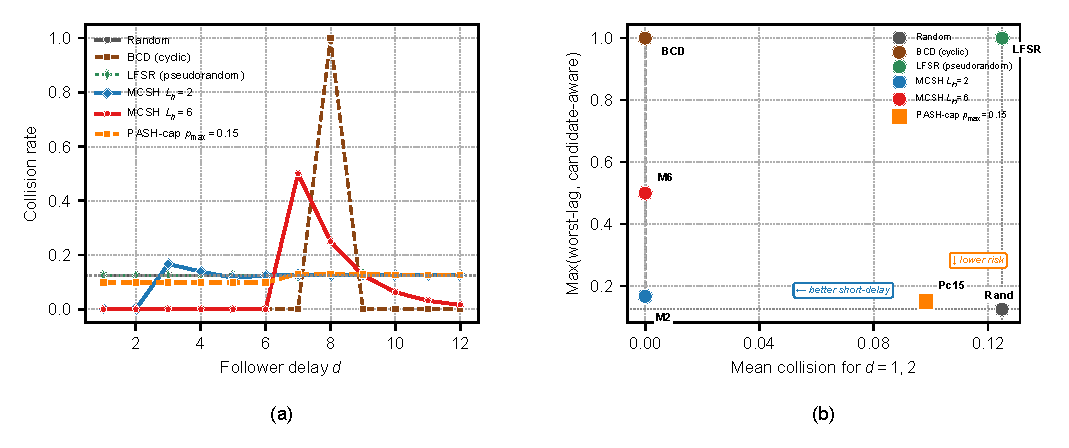
\includegraphics[width=0.96\textwidth]{figures/fig1_structural}
\caption{Structural exposure. (a) MCSH suppresses protected lags but produces
the boundary spike in \eqref{eq:boundary}; PASH-cap limits concentration.
(b) Short-delay protection and worst conditional exposure form a tradeoff.
BCD and LFSR are deterministic stress cases ($R_{\mathrm{cand}}{=}1.0$).}
\label{fig:structural}
\end{figure*}

\section{Boundary Exposure and PASH-Cap}
MCSH with hard memory $L_h$ selects $S$ bins uniformly outside the union of
the $L_h$ most recent active sets whenever feasible. It guarantees
\begin{equation}
\mathcal A_m\cap\mathcal A_{m-d}=\varnothing,\qquad 1\leq d\leq L_h.
\end{equation}
\textbf{Proposition 1 (Boundary spike):} If $(L_h+1)S\leq N$, the collision at the first
unprotected lag is
\begin{equation}
C_{L_h+1}=\frac{S}{N-L_hS}.
\label{eq:boundary}
\end{equation}
\emph{Proof:} By definition, $\mathcal A_m$ is disjoint from each of the
$L_h$ most recent active sets. Under the MCSH rule, each of these $L_h$
sets avoids all predecessors within its own $L_h$-step window, so the
$L_h$ sets that $\mathcal A_m$ excludes are themselves pairwise disjoint.
Together they occupy exactly $L_hS$ distinct bins, leaving $N-L_hS$
unprotected bins from which $\mathcal A_m$ draws uniformly. The historical
set $\mathcal A_{m-L_h-1}$ is at lag $L_h+1$ from $\mathcal A_m$ and is
therefore outside $\mathcal A_m$'s exclusion window. Moreover,
$\mathcal A_{m-L_h-1}$ is disjoint from all of
$\mathcal A_{m-L_h},\ldots,\mathcal A_{m-1}$ (each of these symbols
excludes it through their own $L_h$-step memory). Hence all $S$ of
its elements lie in the unprotected complement. Each such element has
probability $S/(N-L_hS)$ of appearing in the independently drawn
$\mathcal A_m$, giving
\[
C_{L_h+1}=\frac{1}{S}\cdot S\cdot\frac{S}{N-L_hS}=\frac{S}{N-L_hS},
\]
establishing \eqref{eq:boundary}. The expression is strictly increasing in
$L_h$: deeper memory amplifies the very exposure it defers.
$\square$

\textbf{Proposition 2 (Unavoidable predictability cost):} Under MCSH, the
probability-aware exposure equals the boundary-spike height,
\begin{equation}
R_{\mathrm{cand}}=C_{L_h+1}=\frac{S}{N-L_hS}.
\label{eq:cand_mcsh}
\end{equation}
\emph{Proof:} Hard exclusion makes all bins in the unprotected complement
equally likely to be selected, so the conditional inclusion probabilities
$p_{k,m}$ are uniform over that complement (zero for excluded bins, uniform
otherwise). The attacker jams the $S$ bins with largest $p_{k,m}$, all of
which lie in the unprotected complement. The expected fraction of active bins
captured is therefore $S/(N-L_hS)$, matching \eqref{eq:boundary}. $\square$

Proposition~2 identifies a structural lower bound for hard-exclusion
strategies: any rule that guarantees $C_d=0$ for $d\leq L_h$ necessarily
concentrates its conditional probability mass on at most $N-L_hS$
unprotected bins. By the pigeonhole principle, the top-$S$ mass among these
bins cannot have expected value below $S/(N-L_hS)$, and MCSH attains this
lower bound by using the uniform distribution over the unprotected
complement. Any other hard-exclusion rule that deviates from uniformity
would suffer even higher $R_{\mathrm{cand}}$. The designer thus faces an
inescapable tradeoff: zero short-lag collision forces a lower bound on
predictability, and this bound rises sharply as $L_h$ increases, from
$0.143$ at $L_h{=}1$ to $0.500$ at $L_h{=}6$, reaching $1.0$ at $L_h{=}7$ (when $L_hS$ approaches $N$). BCD, a block-cyclic deterministic
construction, illustrates the extreme: perfect short-lag protection
($C_1{=}\cdots{=}C_7{=}0$) but $R_{\mathrm{cand}}{=}1.0$ because of its
periodic structure (usage coefficient of variation (CV) of $0$, max inclusion
probability of $1.0$). In contrast, PASH-cap's $p_{\max}$ bound is
constant; it does not grow with $H$.

PASH-cap replaces hard exclusion with an exponential penalty on recent-use
count. The exponential form keeps the weights strictly positive (avoiding hard
zeros), uses a single parameter $\alpha$, and makes contributions beyond
$H$ steps negligible without explicit truncation. With memory $H$, define
\begin{equation}
w_{k,m}=p_{\mathrm{floor}}+
\exp\!\left[-\alpha\sum_{\ell=1}^{H}\mathbf 1\{k\in\mathcal A_{m-\ell}\}\right].
\end{equation}
The target marginal probabilities are obtained by capped normalization,
\begin{equation}
p_{k,m}=\min\{p_{\max},\eta_m w_{k,m}\},\qquad \sum_{k=1}^{N}p_{k,m}=S,
\label{eq:cap}
\end{equation}
where $\eta_m$ is found by bisection; a solution always exists because
$\sum_k\min(p_{\max},\eta w_{k,m})$ is continuous in $\eta$ with range
$[0,N p_{\max}]\supset[0,S]$.
To realize these marginals exactly, PASH-cap uses fixed-size systematic
sampling: bins are randomly permuted, a uniform offset is drawn, and
bins whose cumulative probability intervals contain any of $S$ equispaced
thresholds are selected. The cap $p_{\max}\leq1$ ensures distinct bins,
and exchangeability under the random permutation guarantees that bin $k$
appears with probability $p_{k,m}$.

For any valid marginals, the probability-aware exposure
\begin{equation}
R_{\mathrm{cand}}=\frac{1}{S}\sum_{k\in\operatorname{TopS}(\boldsymbol p_m)}
p_{k,m}
\label{eq:rcand}
\end{equation}
satisfies $S/N\leq R_{\mathrm{cand}}\leq p_{\max}$; Random attains the lower
bound because all $p_{k,m}=S/N$.

\textbf{Proposition 3 (PASH-cap guaranteed bounds):}
\emph{(i) Candidate-aware exposure:} $R_{\mathrm{cand}}\leq p_{\max}$ for all
$m$ and all history realizations, independent of $H$ and $\alpha$.
\emph{(ii) Self-limiting feedback:} For any bin~$k$ with at least one
appearance in the $H$-step window, its raw weight satisfies
$w_{k,m}\leq p_{\mathrm{floor}}+e^{-\alpha}$. With $\alpha=1.4$,
$e^{-\alpha}\approx0.247$, so two or more appearances reduce the exponential
contribution below~0.061.
\emph{(iii) Self-collision bound:} For any lag $d\geq1$, the self-collision
satisfies $C_d\leq p_{\max}$.

\emph{Proof:} (i) Each $p_{k,m}\leq p_{\max}$ by \eqref{eq:cap}, so the
top-$S$ sum is at most $S\cdot p_{\max}$, yielding the bound.
(ii) When $\sum_{\ell}\mathbf 1\{k\in\mathcal A_{m-\ell}\}\geq1$, the
exponential term is at most $e^{-\alpha}$, so
$w_{k,m}\leq p_{\mathrm{floor}}+e^{-\alpha}$. With $\alpha=1.4$, this is
$0.447$; two or more appearances drop it below $0.261$.
(iii) Let $\mathcal F_m$ denote the history $\mathcal A_{<m}$. The systematic
sampling procedure draws a random permutation independent of $\mathcal F_m$ and
selects bins whose cumulative probability intervals contain equispaced
thresholds. Under the random permutation, each bin $k$ is equally likely to
occupy any position in the permuted order, and the threshold spacing guarantees
$\Pr(k\in\mathcal A_m\mid\mathcal F_m)=p_{k,m}$ (a standard property of randomized systematic sampling; the cap
discussion following \eqref{eq:cap} provides the construction). For any lag $d\geq1$,
\begin{equation}
\begin{aligned}
\Pr(k\in\mathcal A_m\cap\mathcal A_{m-d})
&=\mathbb E\bigl[\mathbf 1\{k\in\mathcal A_{m-d}\}\,
\mathbb E[\mathbf 1\{k\in\mathcal A_m\}\mid\mathcal F_m]\bigr]\\
&=\mathbb E\bigl[\mathbf 1\{k\in\mathcal A_{m-d}\}\,p_{k,m}\bigr]\\
&\leq p_{\max}\,\mathbb E[\mathbf 1\{k\in\mathcal A_{m-d}\}].
\end{aligned}
\label{eq:cd_step}
\end{equation}
By symmetry across bins, each bin has unconditional inclusion probability
$\Pr(k\in\mathcal A_{m-d})=S/N$, so
$\mathbb E[\mathbf 1\{k\in\mathcal A_{m-d}\}]=S/N$. Summing over all $N$ bins
and normalizing by $S$,
\begin{equation}
C_d=\frac{1}{S}\sum_{k=1}^{N}\Pr(k\in\mathcal A_m\cap\mathcal A_{m-d})
\leq\frac{1}{S}\cdot N\cdot p_{\max}\cdot\frac{S}{N}=p_{\max}.
\label{eq:cd_bound}
\end{equation}
The bound requires no approximation and holds for every $d\geq1$ under the
PASH-cap sampling procedure. $\square$

Proposition~3 provides three guarantees that MCSH structurally cannot offer.
Part~(i) bounds the attacker's information advantage against the strongest
probability-aware threat ($R_{\mathrm{cand}}\leq p_{\max}$); part~(ii)
explains the mechanism: a bin appearing even once in the recent window has its
weight bounded by $p_{\mathrm{floor}}+e^{-\alpha}$, preventing the
probability concentration that creates MCSH's boundary spike; part~(iii)
bounds self-collision uniformly ($C_d\leq p_{\max}$), which governs
performance against fixed-delay followers ($d{=}1,3$ in Table~\ref{tab:bler}).
In contrast, MCSH's $C_{L_h+1}=S/(N-L_hS)$ grows toward unity as $L_h$
increases. The bound in part~(iii) is independent of $d$, $H$, and $\alpha$:
it follows solely from the exchangeability of the random permutation and the
per-bin probability cap.
Numerical validation confirms that PASH-cap's worst-case empirical $C_d$ is
$0.131$ (bound $0.15$); the bound is not tight but is uniform over all lags
and independent of $H$ and $\alpha$. The per-bin usage
CV is $0.031$, consistent with long-run uniformity
(versus $0.038$ for Random on the same grid).

\textbf{Remark (Steady-state behavior):} The PASH-cap weight-and-sample
procedure defines a Markov chain on the $H$-step history. Because the
exponential-weight function and the random permutation in systematic
sampling are both label-symmetric, and $p_{\mathrm{floor}}>0$ ensures
that every active-set configuration has positive probability, the
process tends toward an exchangeable steady state in which
$\mathbb E[p_{k,m}]\approx S/N$ for every $k$. With the pointwise bound
$p_{k,m}\leq p_{\max}$ from \eqref{eq:cap}, PASH-cap's per-bin
probabilities are therefore concentrated in the narrow interval
$[S/N,\,p_{\max}]=[0.125,\,0.15]$, independent of $H$. MCSH, by
contrast, assigns probability~0 to $L_hS$ excluded bins and spreads
the remaining mass over the unprotected complement, with its per-bin
maximum $S/(N-L_hS)$ diverging toward~$1.0$ as $L_h\to N/S$. The mixing time is not characterized; the empirical usage CV of $0.031$
(close to Random's $0.038$, see below) indicates near-uniformity within
the simulated horizon. This qualitative contrast explains PASH-cap's
robustness against adaptive and probability-aware attackers.

We use $H=6$, $\alpha=1.4$, $p_{\mathrm{floor}}=0.20$, and $p_{\max}=0.15$.
$H{=}6$ matches MCSH's $L_h{=}6$ for fair comparison; the exponential decay
makes contributions beyond $\sim$5 steps negligible ($e^{-7.0}{\approx}9{\times}10^{-4}$).
With $H{=}0$, weights are uniform and the cap is inactive
($S/N{=}0.125<p_{\max}$); the method reduces to Random.
The per-symbol computation requires $O(NH)$ for weight accumulation and
$O(N+S)$ for sampling. For the tested configuration ($N{=}512$,
$S{=}64$, $H{=}6$), approximately 3000 arithmetic operations per OFDM symbol
are needed, which is negligible relative to typical cyclic-prefix durations.

A structural sweep over
$\alpha\in[0.4,2.0]$, $p_{\mathrm{floor}}\in[0.10,0.35]$,
$p_{\max}\in[0.12,0.20]$ (180~grid points) selected
$(\alpha{=}1.4,p_{\mathrm{floor}}{=}0.20,p_{\max}{=}0.14)$; coded trials
show BLER differs by $<0.005$ across all threats from $p_{\max}{=}0.15$,
which we report for stronger short-delay protection. In the sweep, $p_{\max}$ was dominant ($>0.1$ BLER shift);
$\alpha$ and $p_{\mathrm{floor}}$ had smaller effects ($<0.02$ each).
At 9~dB SNR the ranking is preserved: PASH-cap vs.\ MCSH-L2 is
$0.05$ vs.\ $0.317$ ($d{=}3$) and $0.057$ vs.\ $0.293$ (causal).
A systematic comparison of five online-learning variants
($\epsilon$-greedy at $\epsilon{=}0.10$ and $0.50$, fast adaptation, entropy-regularized, UCB) across four threats confirms this risk: BLER ranges from 0.454 to
1.000, 8.6--23.7$\times$ worse than Random. The candidate-aware
attacker achieves BLER 1.000 against every variant because the learner's
objective (to minimize collision) drives it toward the same low-collision
subcarrier set on every symbol. Once converged, the per-bin usage
distribution becomes extremely concentrated (usage CV $\to 0$, analogous to
BCD's $0.000$), making the conditional marginals deterministic from the
attacker's perspective. This is the structural opposite of PASH-cap, whose
cap-enforced usage CV of $0.031$ remains close to Random's $0.038$.
Online learning without explicit anti-predictability control can be
\emph{worse} than no learning at all, regardless of exploration strategy.

\section{Results}
\label{sec:results}
\subsection{Protocol}
All methods use $N=512$, $S=64$, QPSK, rate-$1/2$ K7 convolutional coding,
mixture-LLR Viterbi receiver, AWGN at 12~dB SNR, 5~dB JSR, and 32-symbol
frames. Coded trials run for at least 2000 frames, stopping after 100 frame
errors or 5000 frames. Bootstrap intervals are descriptive.

\subsection{Structural Mechanism}
Fig.~\ref{fig:structural}(a) confirms \eqref{eq:boundary}. MCSH with
$L_h{=}2$ has $C_1{=}C_2{=}0$, $C_3{\approx}0.167$; $L_h{=}6$ gives
$C_7{=}0.500$, matching Proposition~1. PASH-cap accepts
$C_1{\approx}0.098$ but keeps its worst historical collision ($0.131$) and
$R_{\mathrm{cand}}$ ($0.150$) near Random ($0.125$).
Fig.~\ref{fig:structural}(b) shows MCSH variants on a diagonal where lower
short-delay protection forces higher worst-case risk; PASH-cap occupies a
region inaccessible to hard exclusion.

\begin{figure*}[!t]
\centering
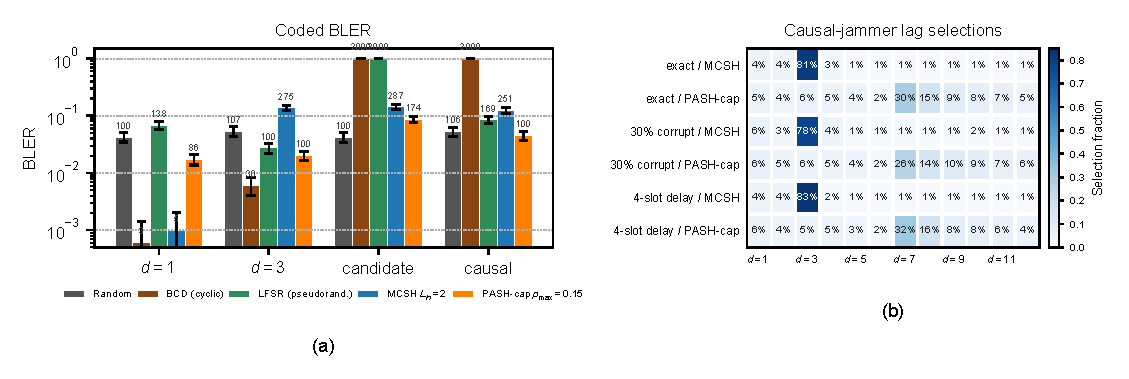
\includegraphics[width=0.96\textwidth]{figures/fig2_coded_feedback}
\caption{Compact coded and feedback results. (a) BLER with descriptive
bootstrap 95\% intervals; numbers above bars are observed frame errors.
(b) Causal-jammer lag-selection fractions under exact, corrupted, and delayed
feedback; each row is normalized independently.}
\label{fig:compact}
\end{figure*}

\subsection{Coded Reliability}
Fig.~\ref{fig:compact}(a) and Table~\ref{tab:bler} show that no rule dominates
every threat. MCSH-L2 is strongest against $d{=}1$ (BLER~0.0010, hard exclusion
eliminates collision) but its own BLER degrades ${\sim}138\times$ from $d{=}1$ to $d{=}3$
(BLER~0.1375) due to the boundary spike. PASH-cap avoids this concentration,
remaining at $0.0200$. Against the causal attacker with 12 candidate lags,
MCSH-L2 sees $>80\%$ of actions concentrated on $d{=}3$ (BLER~0.1255), while
PASH-cap's lag distribution stays diffuse and its BLER of $0.0450$ is near
Random ($0.0530$).

The BLER gap between MCSH-L2 and PASH-cap at $d=3$
($0.1375$ vs.\ $0.0200$, $6.9\times$) far exceeds their collision-rate gap
($0.167$ vs.\ $0.098$, $1.70\times$). This nonlinearity reflects the boundary spike creating collision bursts at
lag $L_h{+}1$ within each frame; the rate-$1/2$ convolutional code
($K{=}7$) has finite memory, so a burst exceeding its correction capability
causes frame loss even at moderate average rates. PASH-cap's soft control
distributes collisions uniformly. The collision-to-BLER mapping is governed
by collision \emph{concentration}, not average rate.

Under full probability awareness, Random achieves the
theoretical lower bound (BLER $0.0422$) because uniform $p_{k,m}$ offers
no concentration to exploit. PASH-cap reaches $0.0870$, substantially
better than MCSH-L2 ($0.1435$).

BCD and an LFSR-based pseudorandom construction further confirm the
phenomenon is not specific to MCSH: BCD has $C_1{=}\cdots{=}C_7{=}0$,
$C_8{=}1.0$, and BLER~1.000 against both adaptive and probability-aware
attackers. LFSR, the classical FH strategy of tactical systems, has
near-Random short-lag BLER (0.0690 at $d{=}1$, 0.0274 at $d{=}3$) and
moderate causal-attacker BLER (0.0845), yet collapses to 1.000 against
the probability-aware attacker because $R_{\mathrm{cand}}{=}1.0$. Any deterministic mapping yields
$p_{k,m}{\in}\{0,1\}$ regardless of implementation, and is fully exploitable.
Two alternative weighting
schemes confirm the exponential form and cap are individually necessary:
PASH-linear (linear decay) improves candidate-aware
BLER to 0.066 but degrades $d{=}1$; PASH-nocap ($p_{\max}{=}1$) improves
$d{=}1$ to 0.006 but suffers candidate-aware BLER 0.354.
\subsection{Feedback Robustness}
Fig.~\ref{fig:compact}(b) shows feedback degradation: MCSH-L2 assigns
80.0\%--83.6\% of actions to $d=3$ under all conditions; the exposure is
structural. PASH-cap keeps lag choices distributed (BLER 0.039--0.047).

\begin{table}[!t]
\centering
\caption{BLER Comparison Across Methods and Threats}
\label{tab:bler}
\footnotesize
\setlength{\tabcolsep}{4.2pt}
\begin{tabular}{lccccc}
\toprule
Threat & Random & BCD & LFSR & MCSH-L2 & PASH-cap \\
\midrule
$d{=}1$  & 0.0425 & \textbf{0.0006} & 0.0690 & 0.0010 & 0.0172 \\
$d{=}3$  & 0.0535 & 0.0060 & 0.0274 & 0.1375 & \textbf{0.0200} \\
Prob.-aware & \textbf{0.0422} & 1.000 & 1.000 & 0.1435 & 0.0870 \\
Causal ($d{\in}\{1,\ldots,12\}$) & 0.0530 & 1.000 & 0.0845 & 0.1255 & \textbf{0.0450} \\
\bottomrule
\end{tabular}

\vspace{3pt}
{\footnotesize Bold = best per row. BCD and LFSR are structural stress cases
($R_{\mathrm{cand}}{=}1.0$): any deterministic hopping rule is fully
exploitable. PASH-cap meets the 100-error target in all rows. Full bootstrap
95\% confidence intervals and supplementary results are available from the
authors.}
\end{table}

\subsection{Scope and Limitations}
Table~\ref{tab:bler} spans the key design dimensions of open-loop
set-valued FH: memoryless stochastic (Random), memoryless deterministic
(BCD, LFSR), memory-based hard exclusion (MCSH), and memory-based soft
exclusion (PASH-cap). BCD and LFSR represent deterministic FH constructions
(whose behavior subsumes that of NHZ sequences naively adapted to
$S{>}1$); the RL matrix represents
closed-loop strategies. External baselines operate under different system
models (wide-gap/NHZ: $S{=}1$; deep-RL: closed-loop state-action spaces)
that preclude faithful reproduction. The comparison isolates
hopping-pattern exposure; it does not claim superiority over published
methods. Attackers have strong information models; bootstrap intervals are
descriptive. AWGN is assumed; fading remains future work.

A simple decision framework emerges: MCSH when the delay is short and
known; PASH-cap when the delay is uncertain or the attacker adapts; Random
when the attacker has full distributional knowledge. PASH-cap fills the
region between these extremes.

\balance
\section{Conclusion}
Avoiding recently used frequencies in anti-jamming FH has an unintended
structural consequence: it concentrates collision risk at the first
unprotected lag. We proved the boundary spike $C_{L_h+1}=S/(N-L_hS)$
follows from the zero-collision guarantee (Proposition~2); deeper memory
amplifies predictability risk. PASH-cap replaces hard exclusion with soft
penalties and a per-subcarrier cap, providing $R_{\mathrm{cand}}{\leq}p_{\max}$
(Proposition~3). The cap is essential: removing it raises candidate-aware
BLER $4.1\times$. BCD and LFSR show the phenomenon is universal: any
deterministic rule has $R_{\mathrm{cand}}{=}1.0$. Five online-learning
variants all fail (BLER 0.454--1.000). Future work includes fading channels
and hardware validation.

\section*{Data Availability}
Code and data available from the authors.

\bibliographystyle{IEEEtran}
\bibliography{references}

\end{document}
